% generated by GAPDoc2LaTeX from XML source (Frank Luebeck)
\documentclass[a4paper,11pt]{report}
\usepackage{tikz}
\usetikzlibrary{positioning}

\usepackage{a4wide}
\sloppy
\pagestyle{myheadings}
\usepackage{amssymb}
\usepackage[latin1]{inputenc}
\usepackage{makeidx}
\makeindex
\usepackage{color}
\definecolor{FireBrick}{rgb}{0.5812,0.0074,0.0083}
\definecolor{RoyalBlue}{rgb}{0.0236,0.0894,0.6179}
\definecolor{RoyalGreen}{rgb}{0.0236,0.6179,0.0894}
\definecolor{RoyalRed}{rgb}{0.6179,0.0236,0.0894}
\definecolor{LightBlue}{rgb}{0.8544,0.9511,1.0000}
\definecolor{Black}{rgb}{0.0,0.0,0.0}

\definecolor{linkColor}{rgb}{0.0,0.0,0.554}
\definecolor{citeColor}{rgb}{0.0,0.0,0.554}
\definecolor{fileColor}{rgb}{0.0,0.0,0.554}
\definecolor{urlColor}{rgb}{0.0,0.0,0.554}
\definecolor{promptColor}{rgb}{0.0,0.0,0.589}
\definecolor{brkpromptColor}{rgb}{0.589,0.0,0.0}
\definecolor{gapinputColor}{rgb}{0.589,0.0,0.0}
\definecolor{gapoutputColor}{rgb}{0.0,0.0,0.0}

%%  for a long time these were red and blue by default,
%%  now black, but keep variables to overwrite
\definecolor{FuncColor}{rgb}{0.0,0.0,0.0}
%% strange name because of pdflatex bug:
\definecolor{Chapter }{rgb}{0.0,0.0,0.0}
\definecolor{DarkOlive}{rgb}{0.1047,0.2412,0.0064}


\usepackage{fancyvrb}

\usepackage{mathptmx,helvet}
\usepackage[T1]{fontenc}
\usepackage{textcomp}


\usepackage[
            pdftex=true,
            bookmarks=true,        
            a4paper=true,
            pdftitle={Written with GAPDoc},
            pdfcreator={LaTeX with hyperref package / GAPDoc},
            colorlinks=true,
            backref=page,
            breaklinks=true,
            linkcolor=linkColor,
            citecolor=citeColor,
            filecolor=fileColor,
            urlcolor=urlColor,
            pdfpagemode={UseNone}, 
           ]{hyperref}

\newcommand{\maintitlesize}{\fontsize{50}{55}\selectfont}

% write page numbers to a .pnr log file for online help
\newwrite\pagenrlog
\immediate\openout\pagenrlog =\jobname.pnr
\immediate\write\pagenrlog{PAGENRS := [}
\newcommand{\logpage}[1]{\protect\write\pagenrlog{#1, \thepage,}}
%% were never documented, give conflicts with some additional packages

\newcommand{\GAP}{\textsf{GAP}}

%% nicer description environments, allows long labels
\usepackage{enumitem}
\setdescription{style=nextline}

%% depth of toc
\setcounter{tocdepth}{1}





%% command for ColorPrompt style examples
\newcommand{\gapprompt}[1]{\color{promptColor}{\bfseries #1}}
\newcommand{\gapbrkprompt}[1]{\color{brkpromptColor}{\bfseries #1}}
\newcommand{\gapinput}[1]{\color{gapinputColor}{#1}}


\begin{document}

\logpage{[ 0, 0, 0 ]}
\begin{titlepage}
\mbox{}\vfill

\begin{center}{\maintitlesize \textbf{\textsf{YAGS}\mbox{}}}\\
\vfill

\hypersetup{pdftitle=\textsf{YAGS}}
\markright{\scriptsize \mbox{}\hfill \textsf{YAGS} \hfill\mbox{}}
{\Huge \textbf{Yet Another Graph System\mbox{}}}\\
\vfill

{\Huge Version 0.0.1\mbox{}}\\[1cm]
{16 February 2016\mbox{}}\\[1cm]
\mbox{}\\[2cm]
{\Large \textbf{R. MacKinney-Romero  \mbox{}}}\\
{\Large \textbf{M.A. Piza{\~n}a   \mbox{}}}\\
{\Large \textbf{ R. Villarroel-Flores   \mbox{}}}\\
\hypersetup{pdfauthor=R. MacKinney-Romero  ; M.A. Piza{\~n}a   ;  R. Villarroel-Flores   }
\end{center}\vfill

\mbox{}\\
{\mbox{}\\
\small \noindent \textbf{R. MacKinney-Romero  }  Email: \href{mailto://rene@xanum.uam.mx} {\texttt{rene@xanum.uam.mx}}}\\
{\mbox{}\\
\small \noindent \textbf{M.A. Piza{\~n}a   }  Email: \href{mailto://mpizana@gmail.com} {\texttt{mpizana@gmail.com}}\\
  Homepage: \href{http://xamanek.izt.uam.mx/map/} {\texttt{http://xamanek.izt.uam.mx/map/}}}\\
{\mbox{}\\
\small \noindent \textbf{ R. Villarroel-Flores   }  Email: \href{mailto://rvf0068@gmail.com} {\texttt{rvf0068@gmail.com}}\\
  Homepage: \href{http://rvf0068.github.io} {\texttt{http://rvf0068.github.io}}}\\
\end{titlepage}

\newpage\setcounter{page}{2}
{\small 
\section*{Copyright}
\logpage{[ 0, 0, 1 ]}
 

\textsf{YAGS} - Yet Another Graph System\\
 Copyright {\copyright} 2016 R. MacKinney-Romero, M.A. Piza{\~n}a and R.
Villarroel-Flores. 

This program is free software: you can redistribute it and/or modify it under
the terms of the GNU General Public License as published by the Free Software
Foundation, either version 3 of the License, or (at your option) any later
version. 

This program is distributed in the hope that it will be useful, but WITHOUT
ANY WARRANTY; without even the implied warranty of MERCHANTABILITY or FITNESS
FOR A PARTICULAR PURPOSE. See the GNU General Public License for more details. 

For details, see the file GPL in the installation directory of \textsf{YAGS} typically under \texttt{GAP-Dir/pkg/yags/GPL} or see \href{http://www.gnu.org/licenses/gpl-3.0.html} {\texttt{http://www.gnu.org/licenses/gpl-3.0.html}}. For contact information see also Section \ref{copyright} in this manual. 

\textsc{Contact information:}\\
 M.A. Piza{\~n}a \\
 \href{mailto://yags@xamanek.izt.uam.mx} {\texttt{yags@xamanek.izt.uam.mx}}\\
 \href{mailto://mpizana@gmail.com} {\texttt{mpizana@gmail.com}}\\
  Departamento de Ingenier{\a'\i}a El{\a'e}ctrica\\
 Universidad Aut{\a'o}noma Metropolitana\\
 Av. San Rafael Atlixco 186.\\
 Col. Vicentina, Del. Iztapalapa\\
 Ciudad de M{\a'e}xico 09340 MEXICO.  \mbox{}}\\[1cm]
\newpage

\def\contentsname{Contents\logpage{[ 0, 0, 2 ]}}

\tableofcontents
\newpage

 
\chapter{\textcolor{Chapter }{Preface}}\label{preface}
\logpage{[ 1, 0, 0 ]}
\hyperdef{L}{X874E1D45845007FE}{}
{
  Ejemplo de cita: \cite{LNP04} 
\section{\textcolor{Chapter }{Disclaimer}}\label{disclaimer}
\logpage{[ 1, 1, 0 ]}
\hyperdef{L}{X7DE9980D7BA36BD1}{}
{
  

\textsc{This is not an official release yet}, this is a version in development. This particular version, 0.0.1, changes
from one day to another without warning and even without a change in the
version number. Also, the operations and global variables can still change
name or even disappear without warning. No commitment is made at the moment
concerning compatibility of this version of the software with any future
version. 

As of this writing (16/Feb/2016) there are only two trustable chapters in this
manual: Appendixes \hyperref[alltopic]{`\textsf{YAGS} Functions by Topic'} and \hyperref[allalpha]{`\textsf{YAGS} Functions Reference'}; also the file \texttt{cheatsheet-yags.pdf} (within directory: \texttt{YAGSDIR/doc/}) may be useful. All other chapters may contain errors, broken links and
misleading information (with higher probability). 

The first official version will be 0.0.2 and is scheduled to be ready this
year (2016), so come back soon. }

 
\section{\textcolor{Chapter }{Welcome to \textsf{YAGS}}}\label{welcometoyags}
\logpage{[ 1, 2, 0 ]}
\hyperdef{L}{X84CD2E0285ABBBC6}{}
{
  

\textsf{YAGS} - \emph{Yet Another Graph System} is a computing system for dealing with graphs, in the sense of Graph Theory
(not bar graphs, pie charts nor graphs of functions). Hence our graphs are
ordered pairs $G=(V,E)$, where $V$ is a finite set of vertices and $E$ is a finite set of edges which are (ordered or unordered) pairs of vertices. 

\textsf{YAGS} was initiated by M.A. Piza{\~n}a in May 2003, and soon incorporated the work
of R. MacKinney-Romero and R. Villarroel-Flores. 

Our motivation here was this and that. 

Our Pourposes and Aim. 

authors, contacts }

 
\section{\textcolor{Chapter }{Citing \textsf{YAGS}}}\label{citingyags}
\logpage{[ 1, 3, 0 ]}
\hyperdef{L}{X792C907981C4DFE4}{}
{
  

If you publish a result and you used \textsf{YAGS} during your research, please cite us as you would normally do with a research
paper:\\
\\
 R. MacKinney-Romero, M.A. Piza{\~n}a and R. Villarroel-Flores.\\
 \emph{YAGS - Yet Another Graph System, Version 0.0.1} (2016)\\
 \href{http://xamanek.izt.uam.mx/yags/} {\texttt{http://xamanek.izt.uam.mx/yags/}}\\
\\
 \texttt{ @manual\texttt{\symbol{123}}YAGS, author = \texttt{\symbol{123}}R.
MacKinney-Romero and M.A. Piza{\~n}a and R.
Villarroel-Flores\texttt{\symbol{125}}, title = \texttt{\symbol{123}}YAGS -
Yet Another Graph System, Version 0.0.1\texttt{\symbol{125}}, year =
\texttt{\symbol{123}}2016\texttt{\symbol{125}}, note =
\texttt{\symbol{123}}http://xamanek.izt.uam.mx/yags/\texttt{\symbol{125}},
\texttt{\symbol{125}} } }

 
\section{\textcolor{Chapter }{Copyright}}\label{copyright}
\logpage{[ 1, 4, 0 ]}
\hyperdef{L}{X81488B807F2A1CF1}{}
{
  

\textsf{YAGS} - Yet Another Graph System\\
 Copyright {\copyright} 2016 R. MacKinney-Romero, M.A. Piza{\~n}a and R.
Villarroel-Flores. 

This program is free software: you can redistribute it and/or modify it under
the terms of the GNU General Public License as published by the Free Software
Foundation, either version 3 of the License, or (at your option) any later
version. 

This program is distributed in the hope that it will be useful, but WITHOUT
ANY WARRANTY; without even the implied warranty of MERCHANTABILITY or FITNESS
FOR A PARTICULAR PURPOSE. See the GNU General Public License for more details. 

For details, see the file GPL in the installation directory of \textsf{YAGS} typically under \texttt{GAP-Dir/pkg/yags/GPL} or see \href{http://www.gnu.org/licenses/gpl-3.0.html} {\texttt{http://www.gnu.org/licenses/gpl-3.0.html}}. 

\textsc{Contact information:}\\
 M.A. Piza{\~n}a \\
 \href{mailto://yags@xamanek.izt.uam.mx} {\texttt{yags@xamanek.izt.uam.mx}}\\
 \href{mailto://mpizana@gmail.com} {\texttt{mpizana@gmail.com}}\\
  Departamento de Ingenier{\a'\i}a El{\a'e}ctrica\\
 Universidad Aut{\a'o}noma Metropolitana\\
 Av. San Rafael Atlixco 186.\\
 Col. Vicentina, Del. Iztapalapa\\
 Ciudad de M{\a'e}xico 09340 MEXICO.  }

 
\section{\textcolor{Chapter }{Authors}}\label{authors}
\logpage{[ 1, 5, 0 ]}
\hyperdef{L}{X7B88101D7EE7EB10}{}
{
  

The authors of \textsf{YAGS} in the chronological order of their first contribution are as follows:\\
\\
 M.A. Piza{\~n}a\\
 Departamento de Ingenier{\a'\i}a El{\a'e}ctrica\\
 Universidad Aut{\a'o}noma Metropolitana\\
 \href{mailto://map@xanum.uam.mx} {\texttt{map@xanum.uam.mx}}\\
\\
 R. MacKinney-Romero\\
 Departamento de Ingenier{\a'\i}a El{\a'e}ctrica\\
 Universidad Aut{\a'o}noma Metropolitana\\
 \href{mailto://rene@xanum.uam.mx} {\texttt{rene@xanum.uam.mx}}\\
\\
 R. Villarroel-Flores\\
 Centro de Investigaci{\a'o}n en Matem{\a'a}ticas\\
 Universidad Aut{\a'o}noma del Estado de Hidalgo\\
 \href{mailto://rafaelv@uaeh.edu.mx} {\texttt{rafaelv@uaeh.edu.mx}} }

 
\section{\textcolor{Chapter }{More Information}}\label{moreinformation}
\logpage{[ 1, 6, 0 ]}
\hyperdef{L}{X80298E137C189819}{}
{
  

More information about \textsf{YAGS} can be found on its official web page: 

`http://xamanek.izt.uam.mx/yags/' 

You can receive notifications about \textsf{YAGS} (i.e. new releases, bug fixes, etc.) by subscribing to its email distribution
list: 

`http://xamanek.izt.uam.mx/cgi-bin/mailman/listinfo/yagsnews/' 

If you are a developer, you may contribute to our project on public
repository: 

`https://github.com/yags/main/' }

 }

 
\chapter{\textcolor{Chapter }{Getting Started}}\label{basics}
\logpage{[ 2, 0, 0 ]}
\hyperdef{L}{X7B1863E17896BCE1}{}
{
  
\section{\textcolor{Chapter }{What is \textsf{YAGS}?}}\label{whatisyags}
\logpage{[ 2, 1, 0 ]}
\hyperdef{L}{X83E7553782F04B65}{}
{
  }

 
\section{\textcolor{Chapter }{Installing \textsf{YAGS}}}\label{installingyags}
\logpage{[ 2, 2, 0 ]}
\hyperdef{L}{X7C143E16864EBAA6}{}
{
  }

 
\section{\textcolor{Chapter }{Testing the Installation}}\label{testingtheinstalation}
\logpage{[ 2, 3, 0 ]}
\hyperdef{L}{X7AE7A7077F513655}{}
{
  }

 
\section{\textcolor{Chapter }{A Gentle Tutorial}}\label{agentletutorial}
\logpage{[ 2, 4, 0 ]}
\hyperdef{L}{X875B75517E6E6576}{}
{
  }

 
\section{\textcolor{Chapter }{An Overview of the Manual}}\label{anoverviewofthemanual}
\logpage{[ 2, 5, 0 ]}
\hyperdef{L}{X80C41AD78251CB64}{}
{
  }

 
\section{\textcolor{Chapter }{Cheatsheet}}\label{cheatsheet}
\logpage{[ 2, 6, 0 ]}
\hyperdef{L}{X7AC1C7197E9E9112}{}
{
  }

 }

 
\chapter{\textcolor{Chapter }{Cliques}}\label{cliques}
\logpage{[ 3, 0, 0 ]}
\hyperdef{L}{X7AA94AAB7961CEC0}{}
{
  
\section{\textcolor{Chapter }{Cliques and Clique Number}}\label{cliquesandcliquenumber}
\logpage{[ 3, 1, 0 ]}
\hyperdef{L}{X786467B78756F151}{}
{
  }

 
\section{\textcolor{Chapter }{Clique Graphs}}\label{cliquegraphs}
\logpage{[ 3, 2, 0 ]}
\hyperdef{L}{X7EC084CC84A85A76}{}
{
  }

 
\section{\textcolor{Chapter }{Basements, Stars and Neckties}}\label{basementsstarsandneckties}
\logpage{[ 3, 3, 0 ]}
\hyperdef{L}{X7E2DB072791C07A4}{}
{
  }

 
\section{\textcolor{Chapter }{Clique Behavior}}\label{cliquebehavior}
\logpage{[ 3, 4, 0 ]}
\hyperdef{L}{X796DE8297FFED431}{}
{
  }

 }

 
\chapter{\textcolor{Chapter }{Graph Categories}}\label{graphcategories}
\logpage{[ 4, 0, 0 ]}
\hyperdef{L}{X7D6C8738844AF8D4}{}
{
  
\section{\textcolor{Chapter }{The Default Graph Category}}\label{thedefaulgraphcategory}
\logpage{[ 4, 1, 0 ]}
\hyperdef{L}{X814CBBB3834F75F2}{}
{
  }

 
\section{\textcolor{Chapter }{The Target Graph Category}}\label{thetargetgraphcategory}
\logpage{[ 4, 2, 0 ]}
\hyperdef{L}{X7871B6627DE80FF8}{}
{
  }

 
\section{\textcolor{Chapter }{Changing the Target Graph Category Temporaryly}}\label{changingthetargetgraphscategorytemporaly}
\logpage{[ 4, 3, 0 ]}
\hyperdef{L}{X7FCC3B977D58AFEB}{}
{
  }

 
\section{\textcolor{Chapter }{Digraphs, Tournaments, etc.}}\label{digraphstournamentsetc}
\logpage{[ 4, 4, 0 ]}
\hyperdef{L}{X816B21B0866ECFEA}{}
{
  }

 }

 
\chapter{\textcolor{Chapter }{Morphisms of Graphs}}\label{morphismsofgraphs}
\logpage{[ 5, 0, 0 ]}
\hyperdef{L}{X7AB9CE86793A0114}{}
{
  
\section{\textcolor{Chapter }{A Quick Start}}\label{aquickstart}
\logpage{[ 5, 1, 0 ]}
\hyperdef{L}{X815230D9851D5961}{}
{
  }

 
\section{\textcolor{Chapter }{Main Procedures}}\label{mainprocedures}
\logpage{[ 5, 2, 0 ]}
\hyperdef{L}{X825944D279109FDC}{}
{
  }

 
\section{\textcolor{Chapter }{User-Defined Types of Morphisms}}\label{userdefinedtypesofmorphisms}
\logpage{[ 5, 3, 0 ]}
\hyperdef{L}{X7A23DC0E7C318B24}{}
{
  }

 
\section{\textcolor{Chapter }{Predefined Types of Morphisms}}\label{predefinedtypesofmorphisms}
\logpage{[ 5, 4, 0 ]}
\hyperdef{L}{X7C6AE3D882EEFFFF}{}
{
  }

 }

 
\chapter{\textcolor{Chapter }{Backtracking}}\label{backtracking}
\logpage{[ 6, 0, 0 ]}
\hyperdef{L}{X82DE80EC7BC3EF58}{}
{
  
\section{\textcolor{Chapter }{A Simple Example}}\label{asimpleexample}
\logpage{[ 6, 1, 0 ]}
\hyperdef{L}{X7F9B599B7C248828}{}
{
  }

 
\section{\textcolor{Chapter }{How Does it Work?}}\label{howdoesitwork}
\logpage{[ 6, 2, 0 ]}
\hyperdef{L}{X81F0E34D8309D890}{}
{
  }

 
\section{\textcolor{Chapter }{Backtracking in Depth}}\label{backtrackingindepth}
\logpage{[ 6, 3, 0 ]}
\hyperdef{L}{X83019AD37D3C77B6}{}
{
  }

 }

 

\appendix


\chapter{\textcolor{Chapter }{\textsf{YAGS} Functions by Topic}}\label{alltopic}
\logpage{[ "A", 0, 0 ]}
\hyperdef{L}{X80E1CB8A7907178D}{}
{
  
\section{\textcolor{Chapter }{Most Common Functions}}\label{tmostcommonfunctions}
\logpage{[ "A", 1, 0 ]}
\hyperdef{L}{X7C2382C381CC357C}{}
{
  }

 
\section{\textcolor{Chapter }{Drawing}}\label{tdrawing}
\logpage{[ "A", 2, 0 ]}
\hyperdef{L}{X7AFE6B467AB077A8}{}
{
  }

 
\section{\textcolor{Chapter }{Constructing Graphs}}\label{tconstructinggraphs}
\logpage{[ "A", 3, 0 ]}
\hyperdef{L}{X865ECABF7952FB46}{}
{
  }

 
\section{\textcolor{Chapter }{Families of Graphs}}\label{tfamilies}
\logpage{[ "A", 4, 0 ]}
\hyperdef{L}{X82B05AAB844DD947}{}
{
  }

 
\section{\textcolor{Chapter }{Small Graphs}}\label{tsmallgraphs}
\logpage{[ "A", 5, 0 ]}
\hyperdef{L}{X870DC04278F413BE}{}
{
  }

 
\section{\textcolor{Chapter }{Attributes and Properties}}\label{tattributesandproperties}
\logpage{[ "A", 6, 0 ]}
\hyperdef{L}{X7DC480E57D26429A}{}
{
  }

 
\section{\textcolor{Chapter }{Unary Operators}}\label{tunaryoperators}
\logpage{[ "A", 7, 0 ]}
\hyperdef{L}{X7F52B61F827F0E83}{}
{
  }

 
\section{\textcolor{Chapter }{Binary Operators}}\label{tbinaryoperators}
\logpage{[ "A", 8, 0 ]}
\hyperdef{L}{X81D9559C7F38A80F}{}
{
  }

 
\section{\textcolor{Chapter }{Cliques}}\label{tcliques}
\logpage{[ "A", 9, 0 ]}
\hyperdef{L}{X7AA94AAB7961CEC0}{}
{
  

Functions dealing with cliques. 
\begin{itemize}
\item \texttt{Basement( \mbox{\texttt{\mdseries\slshape G}}, \mbox{\texttt{\mdseries\slshape KnG}}, \mbox{\texttt{\mdseries\slshape x}} )}\\
 \texttt{Basement( \mbox{\texttt{\mdseries\slshape G}}, \mbox{\texttt{\mdseries\slshape KnG}}, \mbox{\texttt{\mdseries\slshape V}} )}\\
 Returns the basement of vertex \mbox{\texttt{\mdseries\slshape x}} (vertex set \mbox{\texttt{\mdseries\slshape V}}) of the iterated clique graph \mbox{\texttt{\mdseries\slshape KnG}} with respect to \mbox{\texttt{\mdseries\slshape G}}.
\item \texttt{CliqueGraph( \mbox{\texttt{\mdseries\slshape G}} )}\\
 \texttt{CliqueGraph( \mbox{\texttt{\mdseries\slshape G}}, \mbox{\texttt{\mdseries\slshape maxNumCli}} )}\\
 Returns the intersection graph of the (maximal) cliques of \mbox{\texttt{\mdseries\slshape G}}; aborts if \mbox{\texttt{\mdseries\slshape maxNumCli}} cliques are found. 
\item \texttt{CliqueNumber( \mbox{\texttt{\mdseries\slshape G}} )}\\
 Returns the order, $\omega(G)$, of a maximum clique of \mbox{\texttt{\mdseries\slshape G}}. 
\item \texttt{Cliques( \mbox{\texttt{\mdseries\slshape G}} )}\\
 \texttt{Cliques( \mbox{\texttt{\mdseries\slshape G}}, \mbox{\texttt{\mdseries\slshape maxNumCli}} )}\\
 Returns the list of (maximal) cliques of \mbox{\texttt{\mdseries\slshape G}}; aborts if \mbox{\texttt{\mdseries\slshape maxNumCli}} cliques are found. 
\item \texttt{CompletesOfGivenOrder( \mbox{\texttt{\mdseries\slshape G}}, \mbox{\texttt{\mdseries\slshape Ord}} )}\\
 Returns the list of vertex sets of all complete subgraphs of order \mbox{\texttt{\mdseries\slshape Ord}} of \mbox{\texttt{\mdseries\slshape G}}. 
\item \texttt{IsCliqueGated( \mbox{\texttt{\mdseries\slshape G}} )}\\
 Returns `true' if \mbox{\texttt{\mdseries\slshape G}} is a clique gated graph. 
\item \texttt{IsCliqueHelly( \mbox{\texttt{\mdseries\slshape G}} )}\\
 Returns `true' if the set of (maximal) cliques \mbox{\texttt{\mdseries\slshape G}} satisfy the \emph{Helly} property. 
\item \texttt{IsComplete( \mbox{\texttt{\mdseries\slshape G}}, \mbox{\texttt{\mdseries\slshape L}} )}\\
 Returns `true' if \mbox{\texttt{\mdseries\slshape L}} induces a complete subgraph of \mbox{\texttt{\mdseries\slshape G}}.
\item \texttt{IsCompleteGraph( \mbox{\texttt{\mdseries\slshape G}} )}\\
 Returns `true' if graph \mbox{\texttt{\mdseries\slshape G}} is a complete graph, `false' otherwise.
\item \texttt{NumberOfCliques( \mbox{\texttt{\mdseries\slshape G}} )} \\
 \texttt{NumberOfCliques( \mbox{\texttt{\mdseries\slshape G}}, \mbox{\texttt{\mdseries\slshape maxNumCli}} )} \\
 Returns the number of (maximal) cliques of \mbox{\texttt{\mdseries\slshape G}}.
\end{itemize}
 }

 
\section{\textcolor{Chapter }{Morphisms and Isomorphisms}}\label{tmorphismsansisomorphisms}
\logpage{[ "A", 10, 0 ]}
\hyperdef{L}{X7F12235E7845EFB7}{}
{
  }

 
\section{\textcolor{Chapter }{Graphs Categories}}\label{tgraphcategories}
\logpage{[ "A", 11, 0 ]}
\hyperdef{L}{X79AB177982AB8CFA}{}
{
  }

 
\section{\textcolor{Chapter }{Digraphs}}\label{tdigraphs}
\logpage{[ "A", 12, 0 ]}
\hyperdef{L}{X7D554C5D7FDC3D02}{}
{
  }

 
\section{\textcolor{Chapter }{Groups and Rings}}\label{tgroupsandrings}
\logpage{[ "A", 13, 0 ]}
\hyperdef{L}{X7EFF9E2B7F3EBD80}{}
{
  }

 
\section{\textcolor{Chapter }{Backtracking}}\label{tbacktracking}
\logpage{[ "A", 14, 0 ]}
\hyperdef{L}{X82DE80EC7BC3EF58}{}
{
  }

 
\section{\textcolor{Chapter }{Miscellaneous}}\label{tmiscellaneous}
\logpage{[ "A", 15, 0 ]}
\hyperdef{L}{X7C5563A37D566DA5}{}
{
  }

 
\section{\textcolor{Chapter }{Undocumented}}\label{tundocumented}
\logpage{[ "A", 16, 0 ]}
\hyperdef{L}{X86B26CF08302AEF2}{}
{
  }

 }


\chapter{\textcolor{Chapter }{\textsf{YAGS} Functions Reference}}\label{allalpha}
\logpage{[ "B", 0, 0 ]}
\hyperdef{L}{X877A6B7C87471004}{}
{
  This chapter contains a complete list of all \textsf{YAGS}'s functions, with definitions, in alphabetical order. 
\section{\textcolor{Chapter }{Primera seccion}}\label{primera}
\logpage{[ "B", 1, 0 ]}
\hyperdef{L}{X81FB92017A54E6E0}{}
{
                                                                           

\subsection{\textcolor{Chapter }{GraphCategory}}
\logpage{[ "B", 1, 1 ]}\nobreak
\hyperdef{L}{X7D06ED35855A69E1}{}
{\noindent\textcolor{FuncColor}{$\triangleright$\ \ \texttt{GraphCategory({\mdseries\slshape [G, ...]})\index{GraphCategory@\texttt{GraphCategory}}
\label{GraphCategory}
}\hfill{\scriptsize (function)}}\\


 

For internal use. Returns the minimal common category to a list of graphs. If
the list of graphs is empty, the default category is returned. The partial
order (by inclusion) among graph categories is as follows: 

 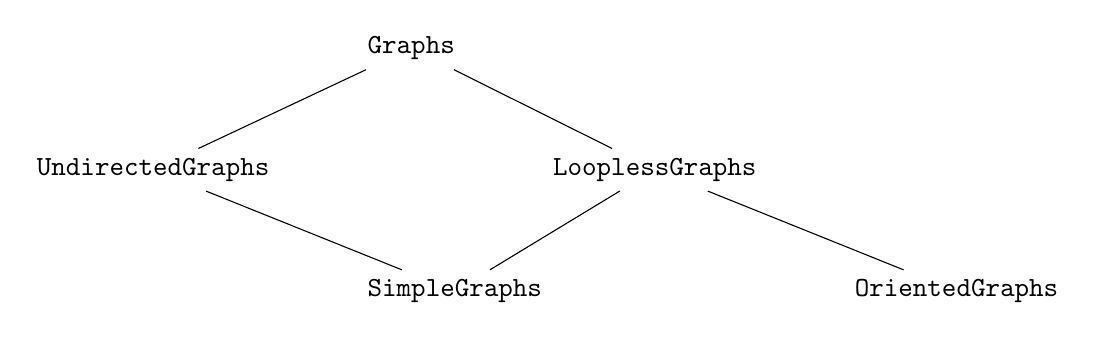
\begin{tikzpicture}[category/.style={font=\ttfamily}] \node (UG) [category]
{UndirectedGraphs}; \node (G) [category, above right=of UG] {Graphs}; \node
(SG) [category, below right=of UG] {SimpleGraphs}; \node (LG) [category, below
right=of G] {LooplessGraphs}; \node (OG) [category, below right=of LG]
{OrientedGraphs}; \draw (UG) -- (G) -- (LG) -- (OG); \draw (UG) -- (SG) --
(LG); \end{tikzpicture}  


\begin{Verbatim}[commandchars=!@|,fontsize=\small,frame=single,label=Example]
  !gapprompt@gap>| !gapinput@g1:=CompleteGraph(2:GraphCategory:=SimpleGraphs);  |
  Graph( Category := SimpleGraphs, Order := 2, Size := 1, Adjacencies := 
  [ [ 2 ], [ 1 ] ] )
  !gapprompt@gap>| !gapinput@g2:=CompleteGraph(2:GraphCategory:=OrientedGraphs);|
  Graph( Category := OrientedGraphs, Order := 2, Size := 1, Adjacencies := 
  [ [ 2 ], [  ] ] )
  !gapprompt@gap>| !gapinput@g3:=CompleteGraph(2:GraphCategory:=UndirectedGraphs);|
  Graph( Category := UndirectedGraphs, Order := 2, Size := 3, Adjacencies := 
  [ [ 1, 2 ], [ 1, 2 ] ] )
  !gapprompt@gap>| !gapinput@GraphCategory([g1,g2,g3]);|
  <Operation "Graphs">
  !gapprompt@gap>| !gapinput@GraphCategory([g1,g2]);   |
  <Operation "LooplessGraphs">
  !gapprompt@gap>| !gapinput@GraphCategory([g1,g3]);|
  <Operation "UndirectedGraphs">
\end{Verbatim}
 }

 

\subsection{\textcolor{Chapter }{Graphs}}
\logpage{[ "B", 1, 2 ]}\nobreak
\hyperdef{L}{X815691877F8C800C}{}
{\noindent\textcolor{FuncColor}{$\triangleright$\ \ \texttt{Graphs\index{Graphs@\texttt{Graphs}}
\label{Graphs}
}\hfill{\scriptsize (filter)}}\\


 \texttt{Graphs} is the most general graph category in \textsf{YAGS}. This category contains all graphs that can be represented in \textsf{YAGS}. A graph in this category may contain loops, arrows and edges (which in \textsf{YAGS} are exactly the same as two opposite arrows between some pair of vertices).
This graph category has no parent category. 
\begin{Verbatim}[commandchars=!@|,fontsize=\small,frame=single,label=Example]
  !gapprompt@gap>| !gapinput@GraphByWalks([1,1],[1,2],[2,1],[3,2]:GraphCategory:=Graphs);|
  Graph( Category := Graphs, Order := 3, Size := 4, Adjacencies := 
  [ [ 1, 2 ], [ 1 ], [ 2 ] ] )
  !gapprompt@gap>| !gapinput@GraphByWalks([1,1],[1,2],[2,1],[3,2]:GraphCategory:=SimpleGraphs);  |
  Graph( Category := SimpleGraphs, Order := 3, Size := 2, Adjacencies := 
  [ [ 2 ], [ 1, 3 ], [ 2 ] ] )
\end{Verbatim}
 }

                                         

\subsection{\textcolor{Chapter }{LooplessGraphs}}
\logpage{[ "B", 1, 3 ]}\nobreak
\hyperdef{L}{X7BD734CC859CDF53}{}
{\noindent\textcolor{FuncColor}{$\triangleright$\ \ \texttt{LooplessGraphs\index{LooplessGraphs@\texttt{LooplessGraphs}}
\label{LooplessGraphs}
}\hfill{\scriptsize (filter)}}\\


 \texttt{LooplessGraphs} is a graph category in \textsf{YAGS}. A graph in this category may contain arrows and edges but no loops. The
parent of this category is \texttt{Graphs}. 
\begin{Verbatim}[commandchars=!@|,fontsize=\small,frame=single,label=Example]
  !gapprompt@gap>| !gapinput@GraphByWalks([1,1],[1,2],[2,1],[3,2]:GraphCategory:=Graphs);|
  Graph( Category := Graphs, Order := 3, Size := 4, Adjacencies := 
  [ [ 1, 2 ], [ 1 ], [ 2 ] ] )
  !gapprompt@gap>| !gapinput@GraphByWalks([1,1],[1,2],[2,1],[3,2]:GraphCategory:=LooplessGraphs);  |
  Graph( Category := LooplessGraphs, Order := 3, Size := 3, Adjacencies := 
  [ [ 2 ], [ 1 ], [ 2 ] ] )
\end{Verbatim}
 }

         

\subsection{\textcolor{Chapter }{Order}}
\logpage{[ "B", 1, 4 ]}\nobreak
\hyperdef{L}{X84F59A2687C62763}{}
{\noindent\textcolor{FuncColor}{$\triangleright$\ \ \texttt{Order({\mdseries\slshape G})\index{Order@\texttt{Order}}
\label{Order}
}\hfill{\scriptsize (attribute)}}\\
\textbf{\indent Returns:\ }
the number of vertices, of graph \mbox{\texttt{\mdseries\slshape G}}.



 
\begin{Verbatim}[commandchars=!@|,fontsize=\small,frame=single,label=Example]
      gap> Order(Icosahedron);
      12
      
\end{Verbatim}
 }

  

\subsection{\textcolor{Chapter }{OrientedGraphs}}
\logpage{[ "B", 1, 5 ]}\nobreak
\hyperdef{L}{X7A5467E379CD8001}{}
{\noindent\textcolor{FuncColor}{$\triangleright$\ \ \texttt{OrientedGraphs\index{OrientedGraphs@\texttt{OrientedGraphs}}
\label{OrientedGraphs}
}\hfill{\scriptsize (filter)}}\\


 \texttt{OrientedGraphs} is a graph category in \textsf{YAGS}. A graph in this category may contain arrows, but no loops or edges. The
parent of this category is \texttt{LooplessGraphs}. 
\begin{Verbatim}[commandchars=!@|,fontsize=\small,frame=single,label=Example]
  !gapprompt@gap>| !gapinput@GraphByWalks([1,1],[1,2],[2,1],[3,2]:GraphCategory:=Graphs);|
  Graph( Category := Graphs, Order := 3, Size := 4, Adjacencies := 
  [ [ 1, 2 ], [ 1 ], [ 2 ] ] )
  !gapprompt@gap>| !gapinput@GraphByWalks([1,1],[1,2],[2,1],[3,2]:GraphCategory:=OrientedGraphs);|
  Graph( Category := OrientedGraphs, Order := 3, Size := 2, Adjacencies := 
  [ [ 2 ], [  ], [ 2 ] ] )
\end{Verbatim}
 }

                          

\subsection{\textcolor{Chapter }{SetDefaulGraphCategory}}
\logpage{[ "B", 1, 6 ]}\nobreak
\hyperdef{L}{X87CEEF1380A6712F}{}
{\noindent\textcolor{FuncColor}{$\triangleright$\ \ \texttt{SetDefaulGraphCategory({\mdseries\slshape Catgy})\index{SetDefaulGraphCategory@\texttt{SetDefaulGraphCategory}}
\label{SetDefaulGraphCategory}
}\hfill{\scriptsize (function)}}\\


 Sets the default graph category to \mbox{\texttt{\mdseries\slshape Catgy}}. The default graph category is used when constructing new graphs when no
other graph category is indicated. New graphs are always forced to comply with
the \texttt{TargetGraphCategory}, so loops may be removed, and arrows may replaced by edges or viceversa,
depending on the category that the new graph belongs to. The available graph
categories are: \texttt{SimpleGraphs}, \texttt{OrientedGraphs}, \texttt{UndirectedGraphs}, \texttt{LooplessGraphs}, and \texttt{Graphs}. 
\begin{Verbatim}[commandchars=!@|,fontsize=\small,frame=single,label=Example]
  !gapprompt@gap>| !gapinput@SetDefaultGraphCategory(Graphs);|
  !gapprompt@gap>| !gapinput@GraphByWalks([1,1],[1,2],[2,1],[3,2]);|
  Graph( Category := Graphs, Order := 3, Size := 4, Adjacencies := 
  [ [ 1, 2 ], [ 1 ], [ 2 ] ] )
  !gapprompt@gap>| !gapinput@SetDefaultGraphCategory(LooplessGraphs);|
  !gapprompt@gap>| !gapinput@GraphByWalks([1,1],[1,2],[2,1],[3,2]);  |
  Graph( Category := LooplessGraphs, Order := 3, Size := 3, Adjacencies := 
  [ [ 2 ], [ 1 ], [ 2 ] ] )
  !gapprompt@gap>| !gapinput@SetDefaultGraphCategory(UndirectedGraphs);|
  !gapprompt@gap>| !gapinput@GraphByWalks([1,1],[1,2],[2,1],[3,2]);    |
  Graph( Category := UndirectedGraphs, Order := 3, Size := 3, Adjacencies := 
  [ [ 1, 2 ], [ 1, 3 ], [ 2 ] ] )
  !gapprompt@gap>| !gapinput@SetDefaultGraphCategory(SimpleGraphs);    |
  !gapprompt@gap>| !gapinput@GraphByWalks([1,1],[1,2],[2,1],[3,2]);|
  Graph( Category := SimpleGraphs, Order := 3, Size := 2, Adjacencies := 
  [ [ 2 ], [ 1, 3 ], [ 2 ] ] )
  !gapprompt@gap>| !gapinput@SetDefaultGraphCategory(OrientedGraphs);|
  !gapprompt@gap>| !gapinput@GraphByWalks([1,1],[1,2],[2,1],[3,2]);  |
  Graph( Category := OrientedGraphs, Order := 3, Size := 2, Adjacencies := 
  [ [ 2 ], [  ], [ 2 ] ] )
\end{Verbatim}
 }

 

\subsection{\textcolor{Chapter }{SimpleGraphs}}
\logpage{[ "B", 1, 7 ]}\nobreak
\hyperdef{L}{X786FE7C97A76D747}{}
{\noindent\textcolor{FuncColor}{$\triangleright$\ \ \texttt{SimpleGraphs\index{SimpleGraphs@\texttt{SimpleGraphs}}
\label{SimpleGraphs}
}\hfill{\scriptsize (filter)}}\\


 \texttt{SimpleGraphs} is a graph category in \textsf{YAGS}. A graph in this category may contain edges, but no loops or arrows. The
category has two parents: \texttt{LooplessGraphs} and \texttt{UndirectedGraphs}. 
\begin{Verbatim}[commandchars=!@|,fontsize=\small,frame=single,label=Example]
  !gapprompt@gap>| !gapinput@GraphByWalks([1,1],[1,2],[2,1],[3,2]:GraphCategory:=Graphs);|
  Graph( Category := Graphs, Order := 3, Size := 4, Adjacencies := 
  [ [ 1, 2 ], [ 1 ], [ 2 ] ] )
  !gapprompt@gap>| !gapinput@GraphByWalks([1,1],[1,2],[2,1],[3,2]:GraphCategory:=SimpleGraphs);  |
  Graph( Category := SimpleGraphs, Order := 3, Size := 2, Adjacencies := 
  [ [ 2 ], [ 1, 3 ], [ 2 ] ] )
\end{Verbatim}
 }

        

\subsection{\textcolor{Chapter }{TargetGraphCategory}}
\logpage{[ "B", 1, 8 ]}\nobreak
\hyperdef{L}{X7F7026FF83934BBC}{}
{\noindent\textcolor{FuncColor}{$\triangleright$\ \ \texttt{TargetGraphCategory({\mdseries\slshape [G, ...]})\index{TargetGraphCategory@\texttt{TargetGraphCategory}}
\label{TargetGraphCategory}
}\hfill{\scriptsize (function)}}\\


 

For internal use. Returns the graph category indicated in the \emph{options stack} if any, otherwise if the list of graphs provided is not empty, returns the
minimal common graph category for the graphs in the list, else returns the
default graph category. The partial order (by inclusion) among graph
categories is as follows: 



 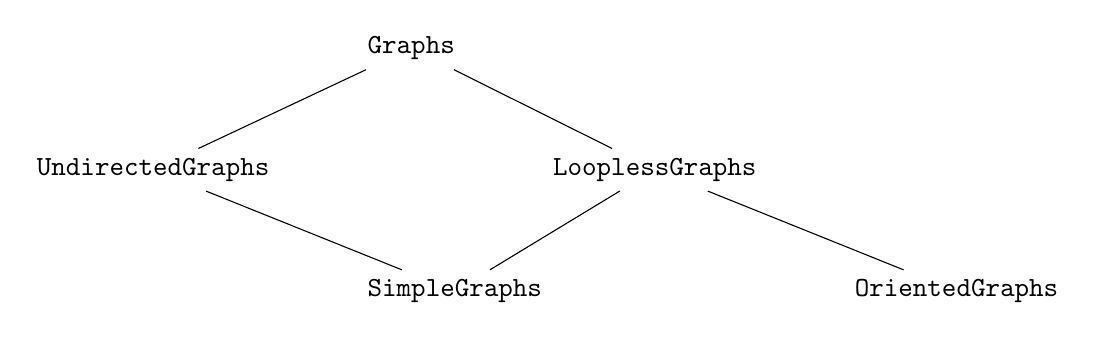
\begin{tikzpicture}[category/.style={font=\ttfamily}] \node (UG) [category]
{UndirectedGraphs}; \node (G) [category, above right=of UG] {Graphs}; \node
(SG) [category, below right=of UG] {SimpleGraphs}; \node (LG) [category, below
right=of G] {LooplessGraphs}; \node (OG) [category, below right=of LG]
{OrientedGraphs}; \draw (UG) -- (G) -- (LG) -- (OG); \draw (UG) -- (SG) --
(LG); \end{tikzpicture}  

This function is internally called by all graph constructing operations in \textsf{YAGS} to decide the graph category that the newly constructed graph is going to
belong to. New graphs are always forced to comply with the \texttt{TargetGraphCategory}, so loops may be removed, and arrows may replaced by edges or viceversa,
depending on the category that the new graph belongs to. 

The \emph{options stack} is a mechanism provided by \textsf{GAP} to pass implicit parameters and is used by \texttt{TargetGraphCategory} so that the user may indicate the graph category she/he wants for the new
graph. 
\begin{Verbatim}[commandchars=!@|,fontsize=\small,frame=single,label=Example]
  !gapprompt@gap>| !gapinput@SetDefaultGraphCategory(SimpleGraphs);             |
  !gapprompt@gap>| !gapinput@g1:=CompleteGraph(2);                              |
  Graph( Category := SimpleGraphs, Order := 2, Size := 1, Adjacencies := 
  [ [ 2 ], [ 1 ] ] )
  !gapprompt@gap>| !gapinput@g2:=CompleteGraph(2:GraphCategory:=OrientedGraphs);|
  Graph( Category := OrientedGraphs, Order := 2, Size := 1, Adjacencies := 
  [ [ 2 ], [  ] ] )
  !gapprompt@gap>| !gapinput@DisjointUnion(g1,g2);|
  Graph( Category := LooplessGraphs, Order := 4, Size := 3, Adjacencies := 
  [ [ 2 ], [ 1 ], [ 4 ], [  ] ] )
  !gapprompt@gap>| !gapinput@DisjointUnion(g1,g2:GraphCategory:=UndirectedGraphs);|
  Graph( Category := UndirectedGraphs, Order := 4, Size := 2, Adjacencies := 
  [ [ 2 ], [ 1 ], [ 4 ], [ 3 ] ] )
\end{Verbatim}
 

In the previous examples, \texttt{TargetGraphCategory} was called internally exactly once for each new graph constructed with the
following parameters: 
\begin{Verbatim}[commandchars=!@|,fontsize=\small,frame=single,label=Example]
  !gapprompt@gap>| !gapinput@TargetGraphCategory();|
  <Operation "SimpleGraphs">
  !gapprompt@gap>| !gapinput@TargetGraphCategory(:GraphCategory:=OrientedGraphs);|
  <Operation "OrientedGraphs">
  !gapprompt@gap>| !gapinput@TargetGraphCategory([g1,g2]);                       |
  <Operation "LooplessGraphs">
  !gapprompt@gap>| !gapinput@TargetGraphCategory([g1,g2]:GraphCategory:=UndirectedGraphs);|
  <Operation "UndirectedGraphs">
\end{Verbatim}
 }

         

\subsection{\textcolor{Chapter }{UndirectedGraphs}}
\logpage{[ "B", 1, 9 ]}\nobreak
\hyperdef{L}{X7CC6D5C77C0CCFA3}{}
{\noindent\textcolor{FuncColor}{$\triangleright$\ \ \texttt{UndirectedGraphs\index{UndirectedGraphs@\texttt{UndirectedGraphs}}
\label{UndirectedGraphs}
}\hfill{\scriptsize (filter)}}\\


 \texttt{UndirectedGraphs} is a graph category in \textsf{YAGS}. A graph in this category may contain edges and loops, but no arrows. The
parent of this category is \texttt{Graphs}. 
\begin{Verbatim}[commandchars=!@|,fontsize=\small,frame=single,label=Example]
  !gapprompt@gap>| !gapinput@GraphByWalks([1,1],[1,2],[2,1],[3,2]:GraphCategory:=Graphs);|
  Graph( Category := Graphs, Order := 3, Size := 4, Adjacencies := 
  [ [ 1, 2 ], [ 1 ], [ 2 ] ] )
  !gapprompt@gap>| !gapinput@GraphByWalks([1,1],[1,2],[2,1],[3,2]:GraphCategory:=UndirectedGraphs);|
  Graph( Category := UndirectedGraphs, Order := 3, Size := 3, Adjacencies := 
  [ [ 1, 2 ], [ 1, 3 ], [ 2 ] ] )
\end{Verbatim}
 }

         }

 }

\def\bibname{References\logpage{[ "Bib", 0, 0 ]}
\hyperdef{L}{X7A6F98FD85F02BFE}{}
}

\bibliographystyle{mapbib}
\bibliography{biblio}

\addcontentsline{toc}{chapter}{References}

\def\indexname{Index\logpage{[ "Ind", 0, 0 ]}
\hyperdef{L}{X83A0356F839C696F}{}
}

\cleardoublepage
\phantomsection
\addcontentsline{toc}{chapter}{Index}


\printindex

\newpage
\immediate\write\pagenrlog{["End"], \arabic{page}];}
\immediate\closeout\pagenrlog
\end{document}
